\documentclass[border=10pt]{standalone}

\usepackage{tikz}
\usepackage{tikzsymbols}
\usetikzlibrary{calc,patterns,shapes.geometric}

\def\centerarc[#1](#2)(#3:#4:#5){\draw[#1] ($(#2)+({#5*cos(#3)},{#5*sin(#3)})$) arc (#3:#4:#5);}

\begin{document}
	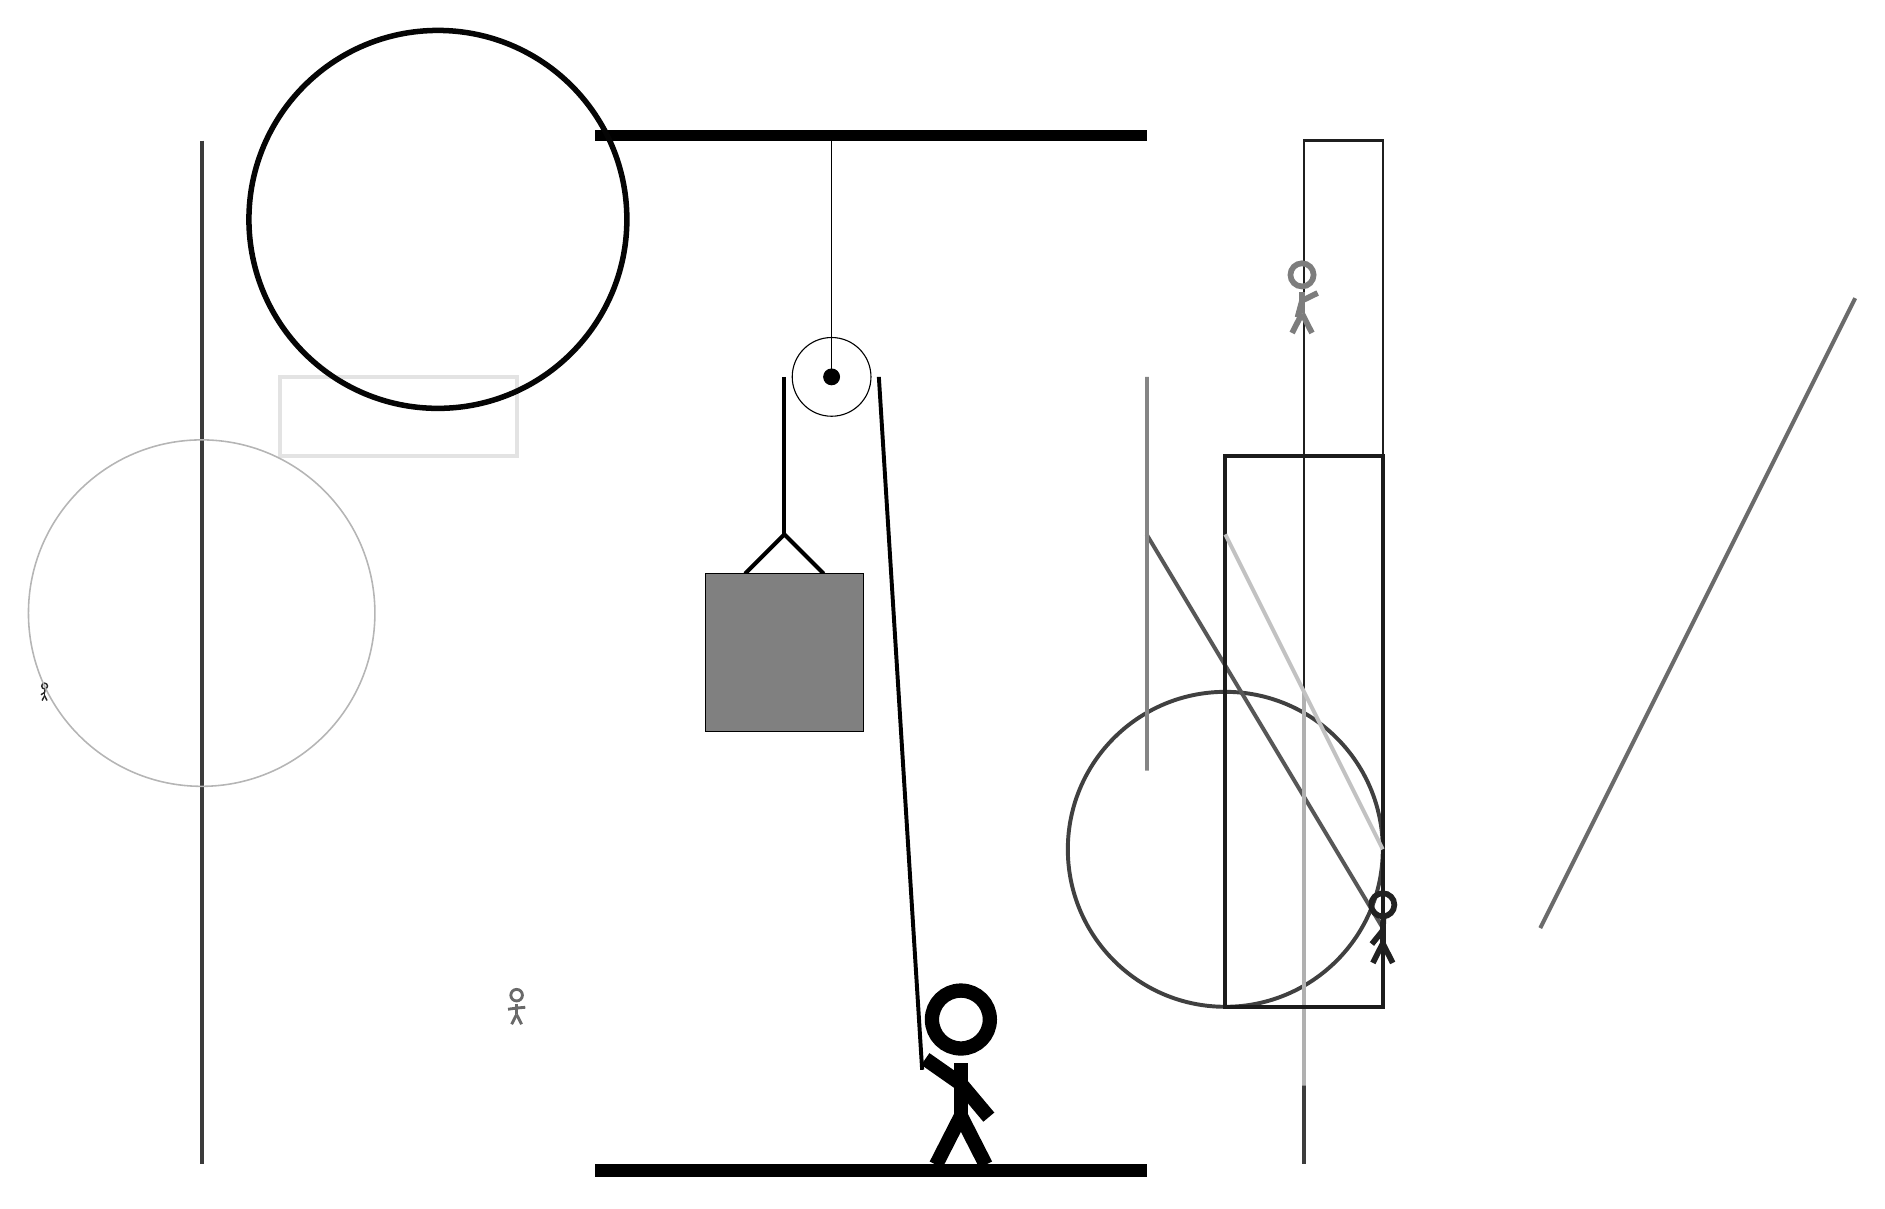
\begin{tikzpicture}
		%%%%% START %%%%%
		
		\draw[fill=black] (-2, 10) rectangle (5, 10.125);
		
		\draw (1, 7) circle (0.5);
		\draw[fill=black] (1, 7) circle (0.1);
		\draw (1, 10) -- (1, 7);
		
		\draw[line width=0.5mm, color=black!58](10, 0) -- (14, 8);
		
		\draw[line width=0.5mm, color=black!11] (-3, 6) rectangle (-6, 7);
		\draw [line width=0.7mm, color=black!98](-4, 9) circle (2.4);
		\draw [line width=0.5mm, color=black!75](6, 1) circle (2.0);
		\draw[line width=0.3mm, color=black!88] (7, 10) rectangle (8, -1);
		
		\node[line width=0.5mm, color=black!59] at (-3, -1) {\Strichmaxerl[2][8][5]};
		
		\node[line width=0.4mm, color=black!85] at (-9, 3) {\Strichmaxerl[1][32][81]};
		\draw[line width=0.5mm, color=black!66](8, 0) -- (5, 5);
		\draw[line width=0.5mm, color=black!76](7, 2) -- (7, -3);
		
		\draw[line width=0.5mm, color=black!48] (5, 2) rectangle (5, 7);
		
		\draw[line width=0.5mm, color=black!77](-7, 10) -- (-7, -3);
		\node[line width=0.5mm, color=black!51] at (7, 8) {\Strichmaxerl[4][75][26]};
		\draw[line width=0.4mm, color=black!31] (7, -2) rectangle (7, 3);
		
		\draw[line width=0.5mm, color=black!89] (6, 6) rectangle (8, -1);
		\draw[line width=0.5mm, color=black!24](6, 5) -- (8, 1);
		\draw [line width=0.2mm, color=black!29](-7, 4) circle (2.2);
		\node[line width=0.3mm, color=black!87] at (8, 0) {\Strichmaxerl[4][51][87]};
		
		\draw[line width=0.5mm] (-0.1, 4.5) -- (0.4, 5.0) -- (0.9, 4.5);
		\draw[fill=black!50] (-0.6, 4.5) rectangle (1.4, 2.5);
		
		\draw[line width=0.5mm] (0.4, 7) -- (0.4, 5.0);
		\centerarc[line width=0.5mm](1, 7)(0:180:0.6);
		\draw[line width=0.5mm](1.6, 7) -- (2.15, -1.8);
		
		\node at (2.6, -1.9) {\Strichmaxerl[10][-35][-50]};
		
		\draw[fill=black] (-2, -3) rectangle (5, -3.15);
		
		%%%%% END %%%%%
	\end{tikzpicture}
\end{document}